\documentclass[a4paper]{article}

\usepackage[utf8]{inputenc}
\usepackage[T1]{fontenc}
\usepackage[croatian]{babel}
\usepackage{url}
\usepackage{amsfonts}
\usepackage{amsmath}
\usepackage{graphicx}

\def\arraystretch{2.0}

\title{Dokumentacija za treću laboratorijsku vježbu iz Računalne~animacije}
\author{Borna~Cafuk}
\date{siječanj~2022.}

\begin{document}

\maketitle

Ovo je dokumentacija za treću laboratorijsku vježbu iz kolegija Računalna animacija. Računalna animacija je kolegij na diplomskom studiju Računarstva na Fakultetu elektrotehnike i računarstva Sveučilišta u Zagrebu.

\section{Upute za pokretanje}

Za izgradnju programa potrebni su programski paketi Node.js i NPM. U direktoriju \texttt{lab3} potrebno pokrenuti je naredbu \texttt{npm install} kako bi se preuzeli i instalirali paketi potrebni za prevođenje i pakiranje programskog koda. Nakon toga treba pokrenuti naredbu \texttt{npm run build:dev} kako bi se program preveo i zapakirao.

U direktoriju \texttt{dist} će se pojaviti datoteke potrebne za pokretanje vježbe. Sadržaj tog direktorija treba servirati nekim HTTP poslužiteljem. Jedan od dostupnih HTTP poslužitelja je u NPM paketu http-server, koji se može koristiti tako da se u direktoriju \texttt{dist} pokrene naredba \texttt{npx http-server}.

Konačno, korištenjem ažurnog i potpunog internetskog preglednika poput Mozilla Firefoxa, Google Chromea ili Microsoft Edgea može se navigirati na mrežnu adresu na kojoj je upogonjen HTTP poslužitelj. Točna adresa će ovisiti o korištenom poslužitelju.

\section{Opis programa}

\begin{figure}[h]
	\caption{Vježba u izvođenju}
	\centering
	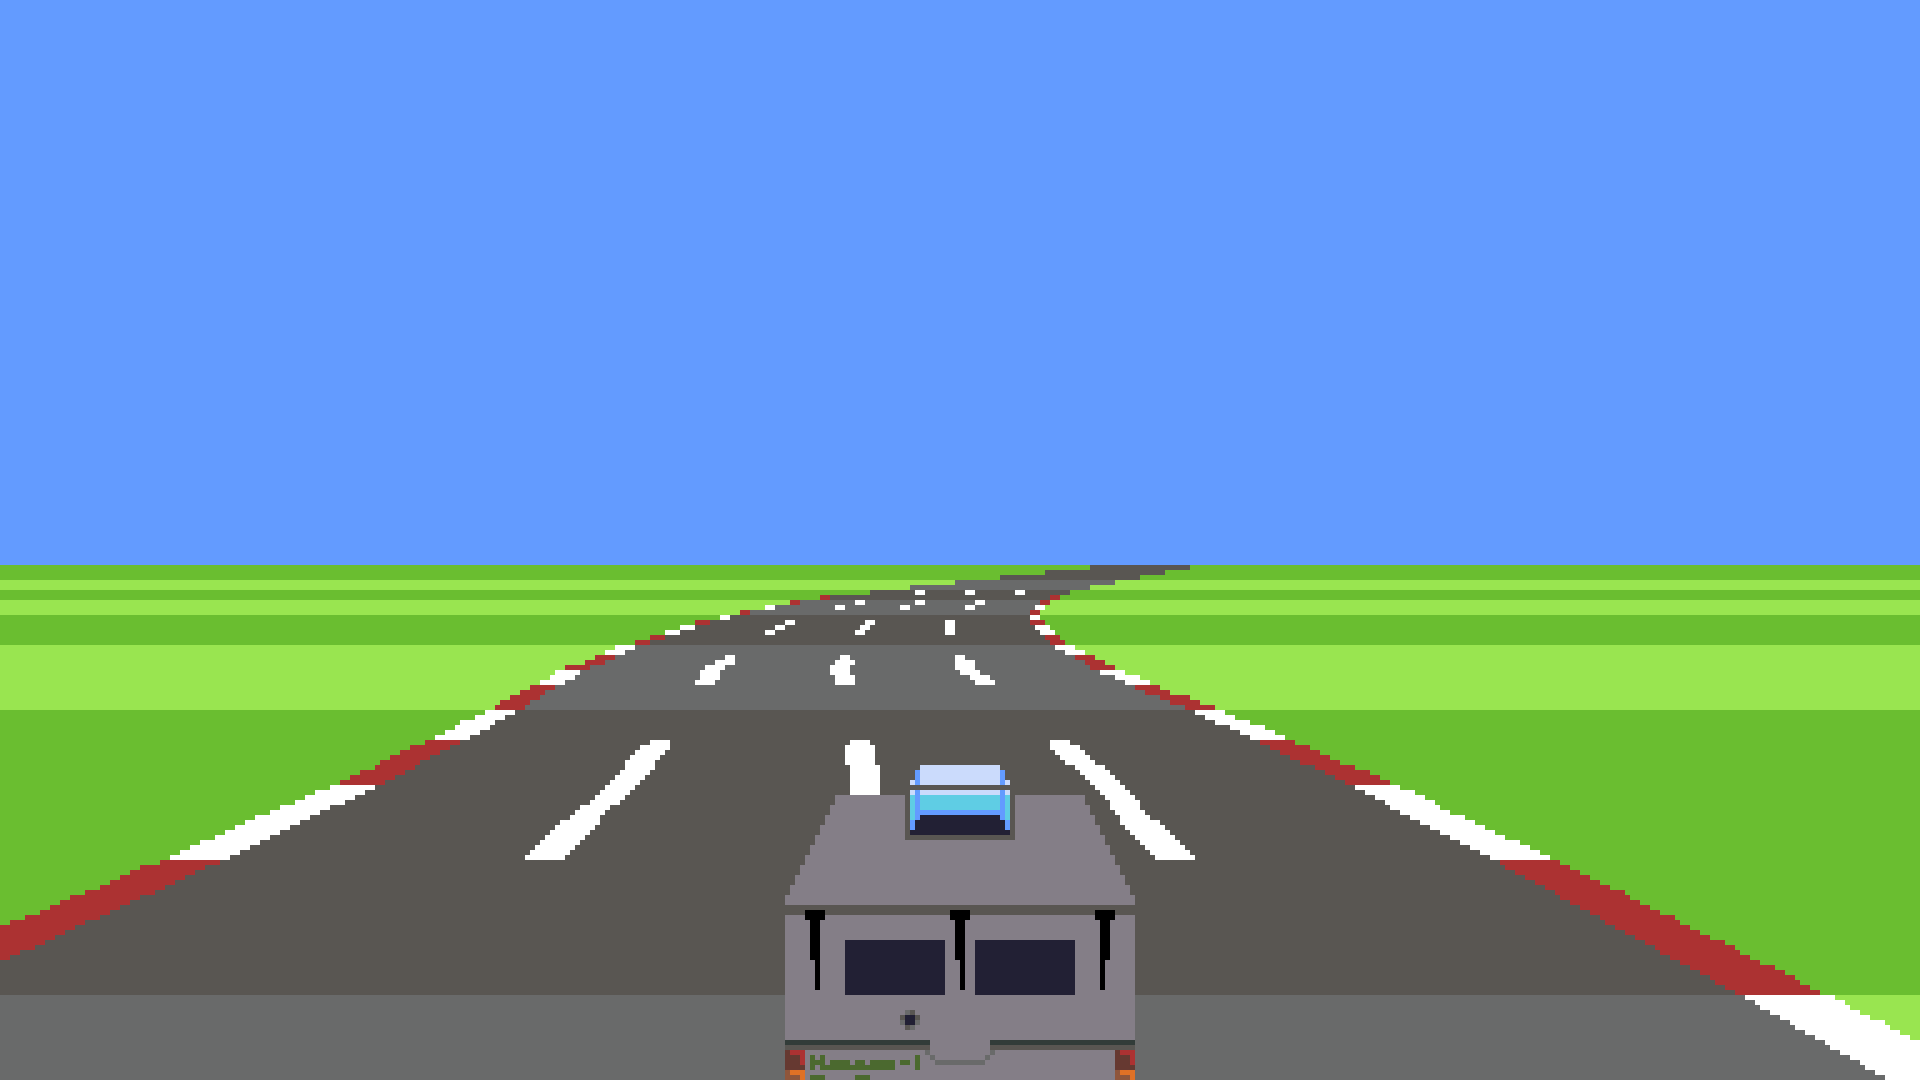
\includegraphics[width=\textwidth]{screenshot}
	\label{fig:screenshot}
\end{figure}

Vježba je nadahnuta arkadnom videoigrom Out Run, koju je 1986. godine proizvela japanska tvrtka Sega. U vježbi je implementiran pseudotrodimenzionalni prikaz ceste i vožnja automobilom duž nje.

U vježbi su oponašane grafičke tehnike korištene u igri Out Run, koje su izvorno korištene zbog ograničenosti tadašnjeg sklopovlja. Ono nije podržavalo matrični račun i koristilo je procesore više redova veličine sporije od onih prisutnih u današnjim stolnim računalima.

Dodatno, upravljanje vozilom u vježbi ostvareno je volanom s papučicama Logitech G29 Driving Force posuđenim sa ZEMRIS\footnote{Zavod za elektroniku, mikroelektroniku, računalne i inteligentne sustave}-a. Volan i papučice se na računalo spajaju USB sučeljem, te su uz instalaciju odgovarajućih upravljačkih programa u operacijskom sustavu vidljivi kao naprava za upravljanje igrama.

Vježba je implementirana u programskom jeziku Typescript, za iscrtavanje se koristi Canvas API, a za dohvat stanja volana i papučica Gamepad API.

\subsection{Definicija oblika ceste}
Cesta je po svojoj dužini podijeljena na segmente jednake duljine. Kamera prati cestu, koja se proteže duž Z-osi. Kako se kamera ne može rotirati, već uvijek gleda u smjeru Z-osi, segmenti ceste mogu biti aproksimirani kao trapezi. Iscrtava se konačan broj segmenata ispred kamere. Svaki segment se iscrtava redak po redak. Oznake na cesti su prikazane tako što se različitim bojama crtaju različiti dijelovi retka, skalirani s obzirom na širinu trapeza u tom retku. Ovisno o indeksu segmenta se te boje mijenjaju kako bi se dobile pruge koje pospješuju percepciju dubine.

U koordinatnom sustavu svijeta se cesta uvijek proteže uz Z-os. Dojam da na cesti postoje zavoji ostvaren je trikom smicanja pojedinih redaka slike na zaslonu. Prividna zakrivljenost ceste definirana je funkcijom $ f \colon \mathbb{R}_{\ge 0} \rightarrow \mathbb{R} $, koja Z-koordinatu preslikava u drugu derivaciju posmaka. Gdje je ona negativna, cesta izgleda kao da skreće ulijevo, a gdje je ona pozitivna, cesta izgleda kao da skreće udesno. Funkcija $ f $ je u kodu definirana po intervalima.

Posmak je definiran sustavom jednadžbi

\begin{equation}
	\left\{\begin{array}{@{}l@{}}
		\dfrac{\mathrm{d}^2 x}{\mathrm{d} z^2} \left( z \right) = f\left( z \right)\\
		\dfrac{\mathrm{d}x}{\mathrm{d}z} \left( z_0 \right) = 0\\
		x \left( z_0 \right) = 0
	\end{array}\right.\,,
\end{equation}

gdje je $z_0$ jednak Z-koordinati prvog vidljivog segmenta. Postupkom integracije se tada dobiva posmak ceste na ekranu, $x \left( z \right)$. Korak integracije odgovara duljini segmenta, a retci između se efektivno linearno interpoliraju zato što se segmenti crtaju kao trapezi.

Konačno, u ovisnosti o vrijednosti funkcije $ f $ se za trenutnu poziciju automobila može grubo simulirati centrifugalna sila koja djeluje na automobil, čime se postiže da on u zavoju skreće s ceste.

Na slici~\ref{fig:exaggerated} je funkcija za crtanje ceste prilagođena na način da parni segmenti budu bijele, a neparni crne boje, kako bi se jasno vidio njihov trapezoidni oblik.

\begin{figure}[h]
	\caption{Slika vježbe s izmijenjenim bojama i povećanom rezolucijom}
	\centering
	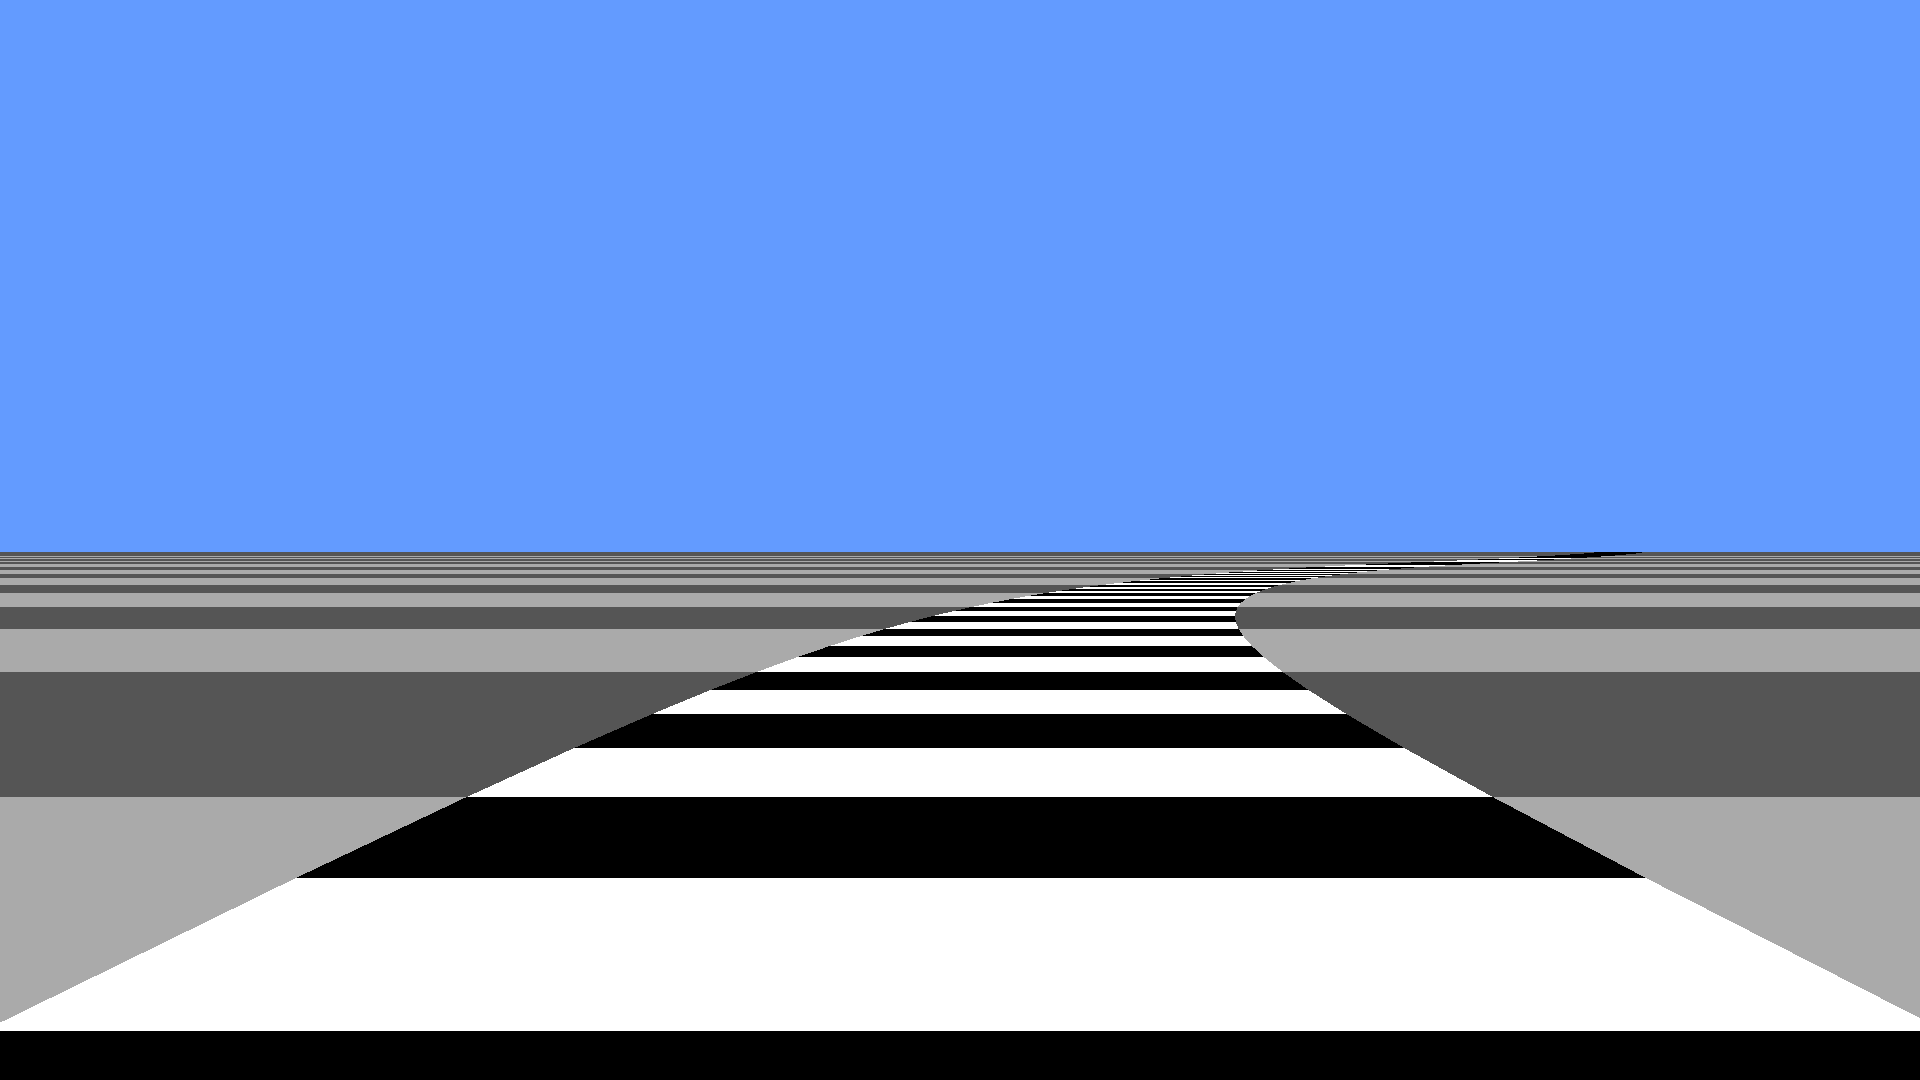
\includegraphics[width=\textwidth]{exaggerated}
	\label{fig:exaggerated}
\end{figure}

\end{document}